\section{Propiedades}



\subsection{El estado de máxima entropía general: dos expresiones}
Sea $\rho\in\mcS(\hilbert_{2})$ caracterizado por tres parámetros: su pureza y dos ángulos, $\alpha$ y $\beta$. Su vector de Bloch se puede escribir entonces como
\begin{equation}
  \vec{r}_{\rho}=r_{\rho}\begin{pmatrix}
    \cos{\beta}\sin{\alpha}\\
    \sin{\beta}\sin{\alpha}\\
    \cos{\alpha}\\
  \end{pmatrix}=r_{\rho}\hat{r}_{\rho} \; \; \; \; \text{con} \; \; \; \; r_{\rho}=\sqrt{2\text{Pu}(\rho)-1}
\end{equation}
Ahora, sea $\rho_{z}\in\mcS(\hilbert_{2})$ un estado solo con componente en $\sigma_{z}$. La unitaria $V$ tal que $V\rho_{z} V^{\dag}$ tiene la forma
\begin{equation}
  V=
  \begin{pmatrix}
      \cos{\frac{\alpha}{2}} & e^{i\beta}\sin{\frac{\alpha}{2}}\\
      -e^{-i\beta}\sin{\frac{\alpha}{2}}& \cos{\frac{\alpha}{2}},
  \end{pmatrix},
\end{equation}
que en términos de la base de Pauli se ve como
\begin{equation}
  V=e^{i\frac{\alpha}{2} \hat{l}\cdot \vec{\sigma}}=\Id \cos{\frac{\alpha}{2}}+i(\hat{l}\cdot \vec{\sigma})\sin{\frac{\alpha}{2}},
\end{equation}
con $\hat{l}=(\sin{\beta},\cos{\beta},0)$, y satisface
\begin{equation}\label{eq:VsigmazV}
  V\sigma_{3}V^{\dag}=\sigma_{1}\cos{\beta}\sin{\alpha}+\sigma_{2}\sin{\beta}\sin{\alpha}+\sigma_{3}\cos{\alpha}=\hat{r}_{\rho}\cdot\vec{\sigma}.
\end{equation}
Construyendo $\mcV=V\otimes V$, podemos expresar al estado de máxima entropía de dos formas equivalentes,
\begin{align}\label{eq:MaxEntTwoExpr}
  \boxed{\varrho_{max}(\rho)=\frac{1}{Z}\text{exp}(-\lambda\mcV\hat{G}_{3}\mcV^{\dag})} && \boxed{\varrho_{max}(\rho)=\frac{1}{Z}\text{exp}(-\sum_{i}\lambda_{i}\hat{G}_{i})}
\end{align} 

\subsection{El estado máxima entropía es separable}

Sea $\rho_{z}$ un estado alineado en $z$ como en (\ref{eq:rhoz}), entonces por (\ref{eq:MaxEnt}) el estado de máxima entropía es:
\begin{equation}\label{eq:MaxEntUgly}
\varrho_{max}^{z}=\frac{1}{Z}\text{exp}(-\lambda\hat{G}_{3}),
\end{equation}
donde $\hat{G}_{3}$ se define según (\ref{eq:Gop}). Como los dos términos que componen al operador comuntan entre sí, la exponencial puede separarse como
\begin{align*}
\varrho_{max}^{z}&=\frac{1}{Z}e^{-\lambda p\sigma_{3}\otimes\Id}e^{-\lambda(1-p)\Id\otimes\sigma_{3}}\\
&=\frac{1}{Z}(e^{-\lambda p\sigma_{3}}\otimes\Id)( \Id\otimes e^{-\lambda(1-p)\sigma_{3}})\\
&=\frac{1}{Z}(e^{-\lambda p\sigma_{3}}\otimes e^{-\lambda(1-p)\sigma_{3}}).\\
\end{align*}
Si se separa a la función de partición como un producto de trazas $Z=Z_{1}Z_{2}$, al estado de máxima entropía se le puede escribir como:
\begin{equation}\label{eq:MaxEntZ}
\varrho_{max}^{z}=\frac{e^{-\lambda p\sigma_{3}}}{Z_{1}} \otimes \frac{e^{-\lambda(1-p)\sigma_{3}}}{Z_{2}}.
\end{equation}
Esto es válido para el estado alineado en $z$, pero retomando el resultado (\ref{eq:MaxEntTwoExpr}) y la relación (\ref{eq:VsigmazV}), el estado de máxima entropía compatible con un estado grueso arbitrario es
\begin{equation}\label{eq:MaxEntSeparable}
  \varrho_{max}=\frac{e^{-\lambda p(\hat{r}_{\rho}\cdot\vec{\sigma})}}{Z_{1}} \otimes \frac{e^{-\lambda(1-p)(\hat{r}_{\rho}\cdot\vec{\sigma})}}{Z_{2}}
\end{equation}
Por lo que el estado de máxima entropía compatible con un estado $\rho$ arbitrario es separable. Ahora, como las expresiones (\ref{eq:MaxEntTwoExpr}) son equivalentes, una vez más, usando (\ref{eq:VsigmazV}) podemos ver que
\begin{align*}
  \sum\lambda_{i}\hat{G}_{i}=&\lambda\mcV(p\sigma_{3}\otimes\Id+(1-p)\Id\otimes\sigma_{3})\mcV^{\dag}\\
  =&\lambda(p(\hat{r}_{\rho}\cdot\vec{\sigma})\otimes\Id+(1-p)\Id\otimes(\hat{r}_{\rho}\cdot\vec{\sigma}))\\
  =& \lambda\sum(\hat{r}_{\rho})_{i}(p\sigma_{i}\otimes\Id+(1-p)\Id\otimes\sigma_{i})\\
  =&\sum_{i}\lambda(\hat{r}_{\rho})_{i}\hat{G}_{i},
\end{align*}
así que
\begin{equation*}
  \lambda_{i}=\lambda(\hat{r}_{\rho})_{i}.
\end{equation*}
De tal forma que (\ref{eq:MaxEntSeparable}) puede escribirse en términos de los tres multiplicadores de Lagrange como:
\begin{equation*}
\varrho_{max}=\frac{e^{-p\sum_{i}\lambda_{i}\sigma_{i}}}{Z_{1}} \otimes \frac{e^{-(1-p)\sum_{i}\lambda_{i}\sigma_{i}}}{Z_{2}}
\end{equation*}
¿Qué significa que el estado de máxima entropía sea separable? ¿Qué interpretación tienen las matrices de densidad reducidad del estado de máxima entropía? La propiedad de separabilidad viene de que la información accesible al experimentalista no incluye las correlaciones entre los subsistemas. Los observables finos son combinaciones de operadores de la forma $\pauli{i}\otimes\Id$ y $\Id\otimes\pauli{j}$. Esto significa que lo que se reconstruye es una combinación lineal de las matrices de densidad reducidas correspondientes a cada subsistema. Por la construcción de la aplicación de grano grueso, cualquier sistema de matrices de densidad reducidas $\rho_{A}$ y $\rho_{B}$ da como resultado el mismo estado efectivo, sin importar qué tan factorizable o entrelazado esté (de nuevo, siempre y cuando las marices de densidad reducidas sean $\rho_{A}$ y $\rho_{B}$). Pues bien, como estas correlaciones se pierden a la hora de hacer las mediciones, en el estado de máxima entropía estas se hacen cero. En el caso estacionario esto no afecta, pero me preocupa que quizá no sea el mejor acercamiento para el caso dinámico. Me pregunto si habrá algo como una dinámica de máxima entropía. 

Algo que queda en claro de esto es que el estado de máxima entropía es completamente dependiente de los observables que se usen en su contrucción. Después de todo, la maximización de la entropía se restringe de acuerdo a las observaciones experimentales, así que estados de máxima entropía que cumplan un conjunto particular de restricciones no tienen por qué (y probablemente no lo harán) satisfacer un conjunto diferente de restricciones, un conjunto mediante el cual se contruiría un estado de máxima entropía diferente.

Hay algo interesante, y es que para el caso clásico, la distribución de máxima entropía parece converger a la distribución real cuando se conocen una infinidad de sus momentos. No lo he probado, y no lo haré, pero me parece importante escribirlo para tenerlo en mente.

Ahora se usan dos cosas: que $\sum_{i}\lambda_{i}\sigma_{i}=\lambda(\hat{r}_{\rho}\cdot\vec{\sigma})$ con $\lambda=\sqrt{\sum \lambda_{i}^{2}}$, y que podemos subir $p$ y $(1-p)$ como potencias, así que
\begin{align*}
  \varrho_{max}=&\frac{e^{-p\sum_{i}\lambda_{i}\sigma_{i}}}{Z_{1}} \otimes \frac{e^{-(1-p)\sum_{i}\lambda_{i}\sigma_{i}}}{Z_{2}}\\
  =&\frac{\qty(e^{-\sum_{i}\lambda_{i}\sigma_{i}})^{p} }{Z_{1}}\otimes \frac{\qty(e^{-\sum_{i}\lambda_{i}\sigma_{i}})^{1-p}}{Z_{2}}\\
  =&\frac{\qty(e^{-\lambda(\hat{r}_{\rho}\cdot\vec{\sigma})})^{p}}{Z_{1}} \otimes \frac{\qty(e^{-\lambda(\hat{r}_{\rho}\cdot\vec{\sigma})})^{1-p}}{Z_{2}}\\
\end{align*}
Expandiendo en la base de pauli, y factorizando un $\cosh{\lambda}$:
\begin{align*}
  \varrho_{max}=&\frac{\qty(\cosh{\lambda}(\Id-\tanh{\lambda}(\hat{r}_{\rho}\cdot\vec{\sigma})))^{p}}{\Tr[\qty(\cosh{\lambda}(\Id-\tanh{\lambda}(\hat{r}_{\rho}\cdot\vec{\sigma})))^{p}]} \otimes \frac{\qty(\cosh{\lambda}(\Id-\tanh{\lambda}(\hat{r}_{\rho}\cdot\vec{\sigma})))^{1-p}}{\Tr[\qty(\cosh{\lambda}(\Id-\tanh{\lambda}(\hat{r}_{\rho}\cdot\vec{\sigma})))^{1-p}]}\\
  =&\frac{\qty(\Id-\tanh{\lambda}(\hat{r}_{\rho}\cdot\vec{\sigma}))^{p}}{\Tr[\qty(\Id-\tanh{\lambda}(\hat{r}_{\rho}\cdot\vec{\sigma}))^{p}]} \otimes \frac{\qty(\Id-\tanh{\lambda}(\hat{r}_{\rho}\cdot\vec{\sigma}))^{1-p}}{\Tr[\qty(\Id-\tanh{\lambda}(\hat{r}_{\rho}\cdot\vec{\sigma}))^{1-p}]}
\end{align*}
Definimos
\begin{equation}
  \boxed{\rho_{max}=\frac{1}{2}(\Id-\tanh{\lambda}(\hat{r}_{\rho}\cdot\vec{\sigma}))}
\end{equation}
de tal manera que 
\begin{equation}\label{eq:MaxEntSeparableLM}
  \boxed{\varrho_{max}=\frac{(\rho_{max})^{p}}{\Tr[ (\rho_{max})^{p}]}\otimes\frac{(\rho_{max})^{1-p}}{\Tr[(\rho_{max})^{1-p}]}}
\end{equation}

\subsection{El estado de máxima entropía bajo la aplicación de grano grueso}\label{sec:CG(MaxEnt)}
El problema de la ecuación (\ref{eq:MaxEntSeparable}) es que el estado de máxima entropía está en términos de los multiplicadores de Lagrange (en particular, de $\lambda$), en lugar de cantidades medibles. Si por alguna razón tuviéramos que resignarnos a trabajar con el estado en términos de $\lambda$, será necesario conocer la expresión del estado efectivo. Para hallarla, basta con pasar (\ref{eq:MaxEntSeparableLM}) por la aplicación de grano grueso.
\begin{equation}\label{eq:CG(MaxEntZ)1}
    \rho=\frac{1}{Z}\CG{\varrho_{max}}=p\frac{e^{-\lambda p(\hat{r}_{\rho}\cdot\vec{\sigma})}}{Z_{1}}+(1-p)\frac{e^{-\lambda (1-p)(\hat{r}_{\rho}\cdot\vec{\sigma})}}{Z_{2}}.
\end{equation}
Sustituyendo
\begin{equation}\label{eq:PauliVectorExp}
    e^{a\hat{n}\cdot \vec{\sigma}}=\Id \cosh{a}+(\hat{n}\cdot \vec{\sigma})\sinh{a}.
\end{equation}
¿en (\ref{eq:CG(MaxEntZ)1}) se encuentra la expresión del estado efectivo en términos de la base de Pauli
\begin{align*}
    \rho_{z}&=p\frac{\Id \cosh{\lambda p}-(\hat{r}_{\rho}\cdot\vec{\sigma})\sinh{\lambda p}}{Z_{1}}+(1-p)\frac{\Id \cosh{\lambda (1-p)}-(\hat{r}_{\rho}\cdot\vec{\sigma})\sinh{\lambda (1-p)}}{Z_{2}}\\
    &=p\frac{1}{2}(\Id \frac{2\cosh{\lambda p}}{Z_{1}}-(\hat{r}_{\rho}\cdot\vec{\sigma})\frac{2\sinh{\lambda p}}{Z_{1}})+(1-p)\frac{1}{2}(\Id \frac{2\cosh{\lambda (1-p)}}{Z_{2}}-(\hat{r}_{\rho}\cdot\vec{\sigma})\frac{2\sinh{\lambda (1-p)}}{Z_{2}}).
\end{align*}
Para que esto sea de la forma $\rho=\sum_{i}p_{i}\rho_{i}$ es necesario que $Z_{1}=2\cosh{\lambda p}$ y $Z_{2}=2\cosh{\lambda (1-p)}$ (cosa que se puede comprobar). El estado efectivo en términos de $\lambda $ es
\begin{equation}\label{eq:CG(MaxEntZ)2}
    \rho_{z}=p\frac{1}{2}(\Id+(\hat{r}_{\rho}\cdot\vec{\sigma})\tanh{(-\lambda p)})+(1-p)\frac{1}{2}(\Id+(\hat{r}_{\rho}\cdot\vec{\sigma})\tanh{(-\lambda (1-p))}).
\end{equation}
juntando los términos
\begin{equation}\label{eq:CG(MaxEnt)}
  \boxed{\rho=\frac{1}{2}[\Id+(\hat{r}_{\rho}\cdot\vec{\sigma})(p\tanh{-\lambda p}+(1-p)\tanh{-\lambda (1-p)})]}
\end{equation}
Todo lo anterior nos permite obtener otra expresión para $\varrho_{max}$:
\begin{equation*}
  \varrho_{max}=\frac{1}{2}(\Id+(\hat{r}_{\rho}\cdot\vec{\sigma})\tanh{(-\lambda p)})\otimes\frac{1}{2}(\Id+(\hat{r}_{\rho}\cdot\vec{\sigma})\tanh{(-\lambda (1-p))})
\end{equation*}
\subsection{El estado de máxima entropía en términos de la pureza}

La ecuación (\ref{eq:CG(MaxEnt)}) permite expresar la pureza $\text{Pu}(\rho)$ en términos de $\lambda$. Recordando que $\text{Pu}(\rho)=\frac{1}{2}(r_{\rho}^{2}+1)$,
\begin{equation}\label{eq:RzTanh}
    \boxed{r_{\rho}=-(p\tanh{\lambda p}+(1-p)\tanh{\lambda (1-p)})}  
\end{equation}
La ecuación anterior, fijada $p$, es una suma de dos funciones inyectivas, y como tal, es inyectiva también. Esto significa que existe la función inversa. La figura \ref{fig:rzinv} muestra la forma de $r_{\rho}(\lambda)$ para valores selectos de $p$. Después de una breve inspección de (\ref{eq:RzTanh}) se concluyen las siguientes cosas:
\begin{itemize}
\item la superficie es simétrica respecto al plano $p=0.5$
\item la superficie es antisimétrica  respecto al plano $\lambda=0$ i.e. $r_{\rho}(\lambda,p)=-r_{\rho}(-\lambda,p)$
\item $\text{sgn}(\lambda)=-\text{sgn}(r_{\rho})$
\end{itemize}
\begin{figure}[h!]
\centering
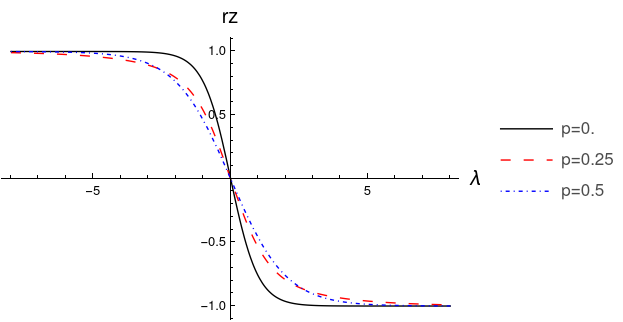
\includegraphics[width=0.6\linewidth]{maxent/figures/rz(lambda)_lambda-8to8.png}
\caption{$r_{\rho}$ como función de $\lambda$ para diferentes valores de $q$. La apariencia uno a uno sugiere la existencia de una inversa.}
\label{fig:rzinv}
\end{figure}

\subsubsection{Dos soluciones particulares}

Considerando el caso $p=0$ o $p=1$, la ecuación (\ref{eq:RzTanh}) se reduce a 
\begin{equation}
r_{\rho}=-\tanh{\lambda}
\end{equation}
de manera que $\lambda=-\text{arctanh}(r_{\rho})$.

Si $p=\frac{1}{2}$, la ecuación (\ref{eq:RzTanh}) se reduce a
\begin{equation}
r_{\rho}=-\tanh\frac{1}{2}\lambda
\end{equation}
de manera que $\lambda=-\text{arctanh}(2r_{z})$.
En el límite $(1-p)\rightarrow 0$,
\begin{equation}
  r_{\rho}=-(\tanh{\lambda}+p(\lambda\sech^{2}{\lambda}+\tanh{\lambda}))
\end{equation}
\newpage